\newpage
\section{Joulemeter}
The purpose of this block is to be able to measure the energy consumed by the Propulsion Motor. This block differs from the other blocks in that it is only a part of the system during the Shell Eco-Marathon. As the Joulemeter is property of Shell this documentation will not contain any unity test of the block.

\subsection{Analysis}
According to the SEM rules the Joulemeter must measure the energy delivered from the Battery to the Propulsion Motor. The Joulemeter must therefore be located between the Battery and the Power Control-Block (which in turn is located in the Motor Control System). It is very important that the joulemeter doesn't measure energy which isn't consumed by the motor. Thus the following Energy Supply Diagram can be constructed:

\begin{figure}[H]
	\centering
	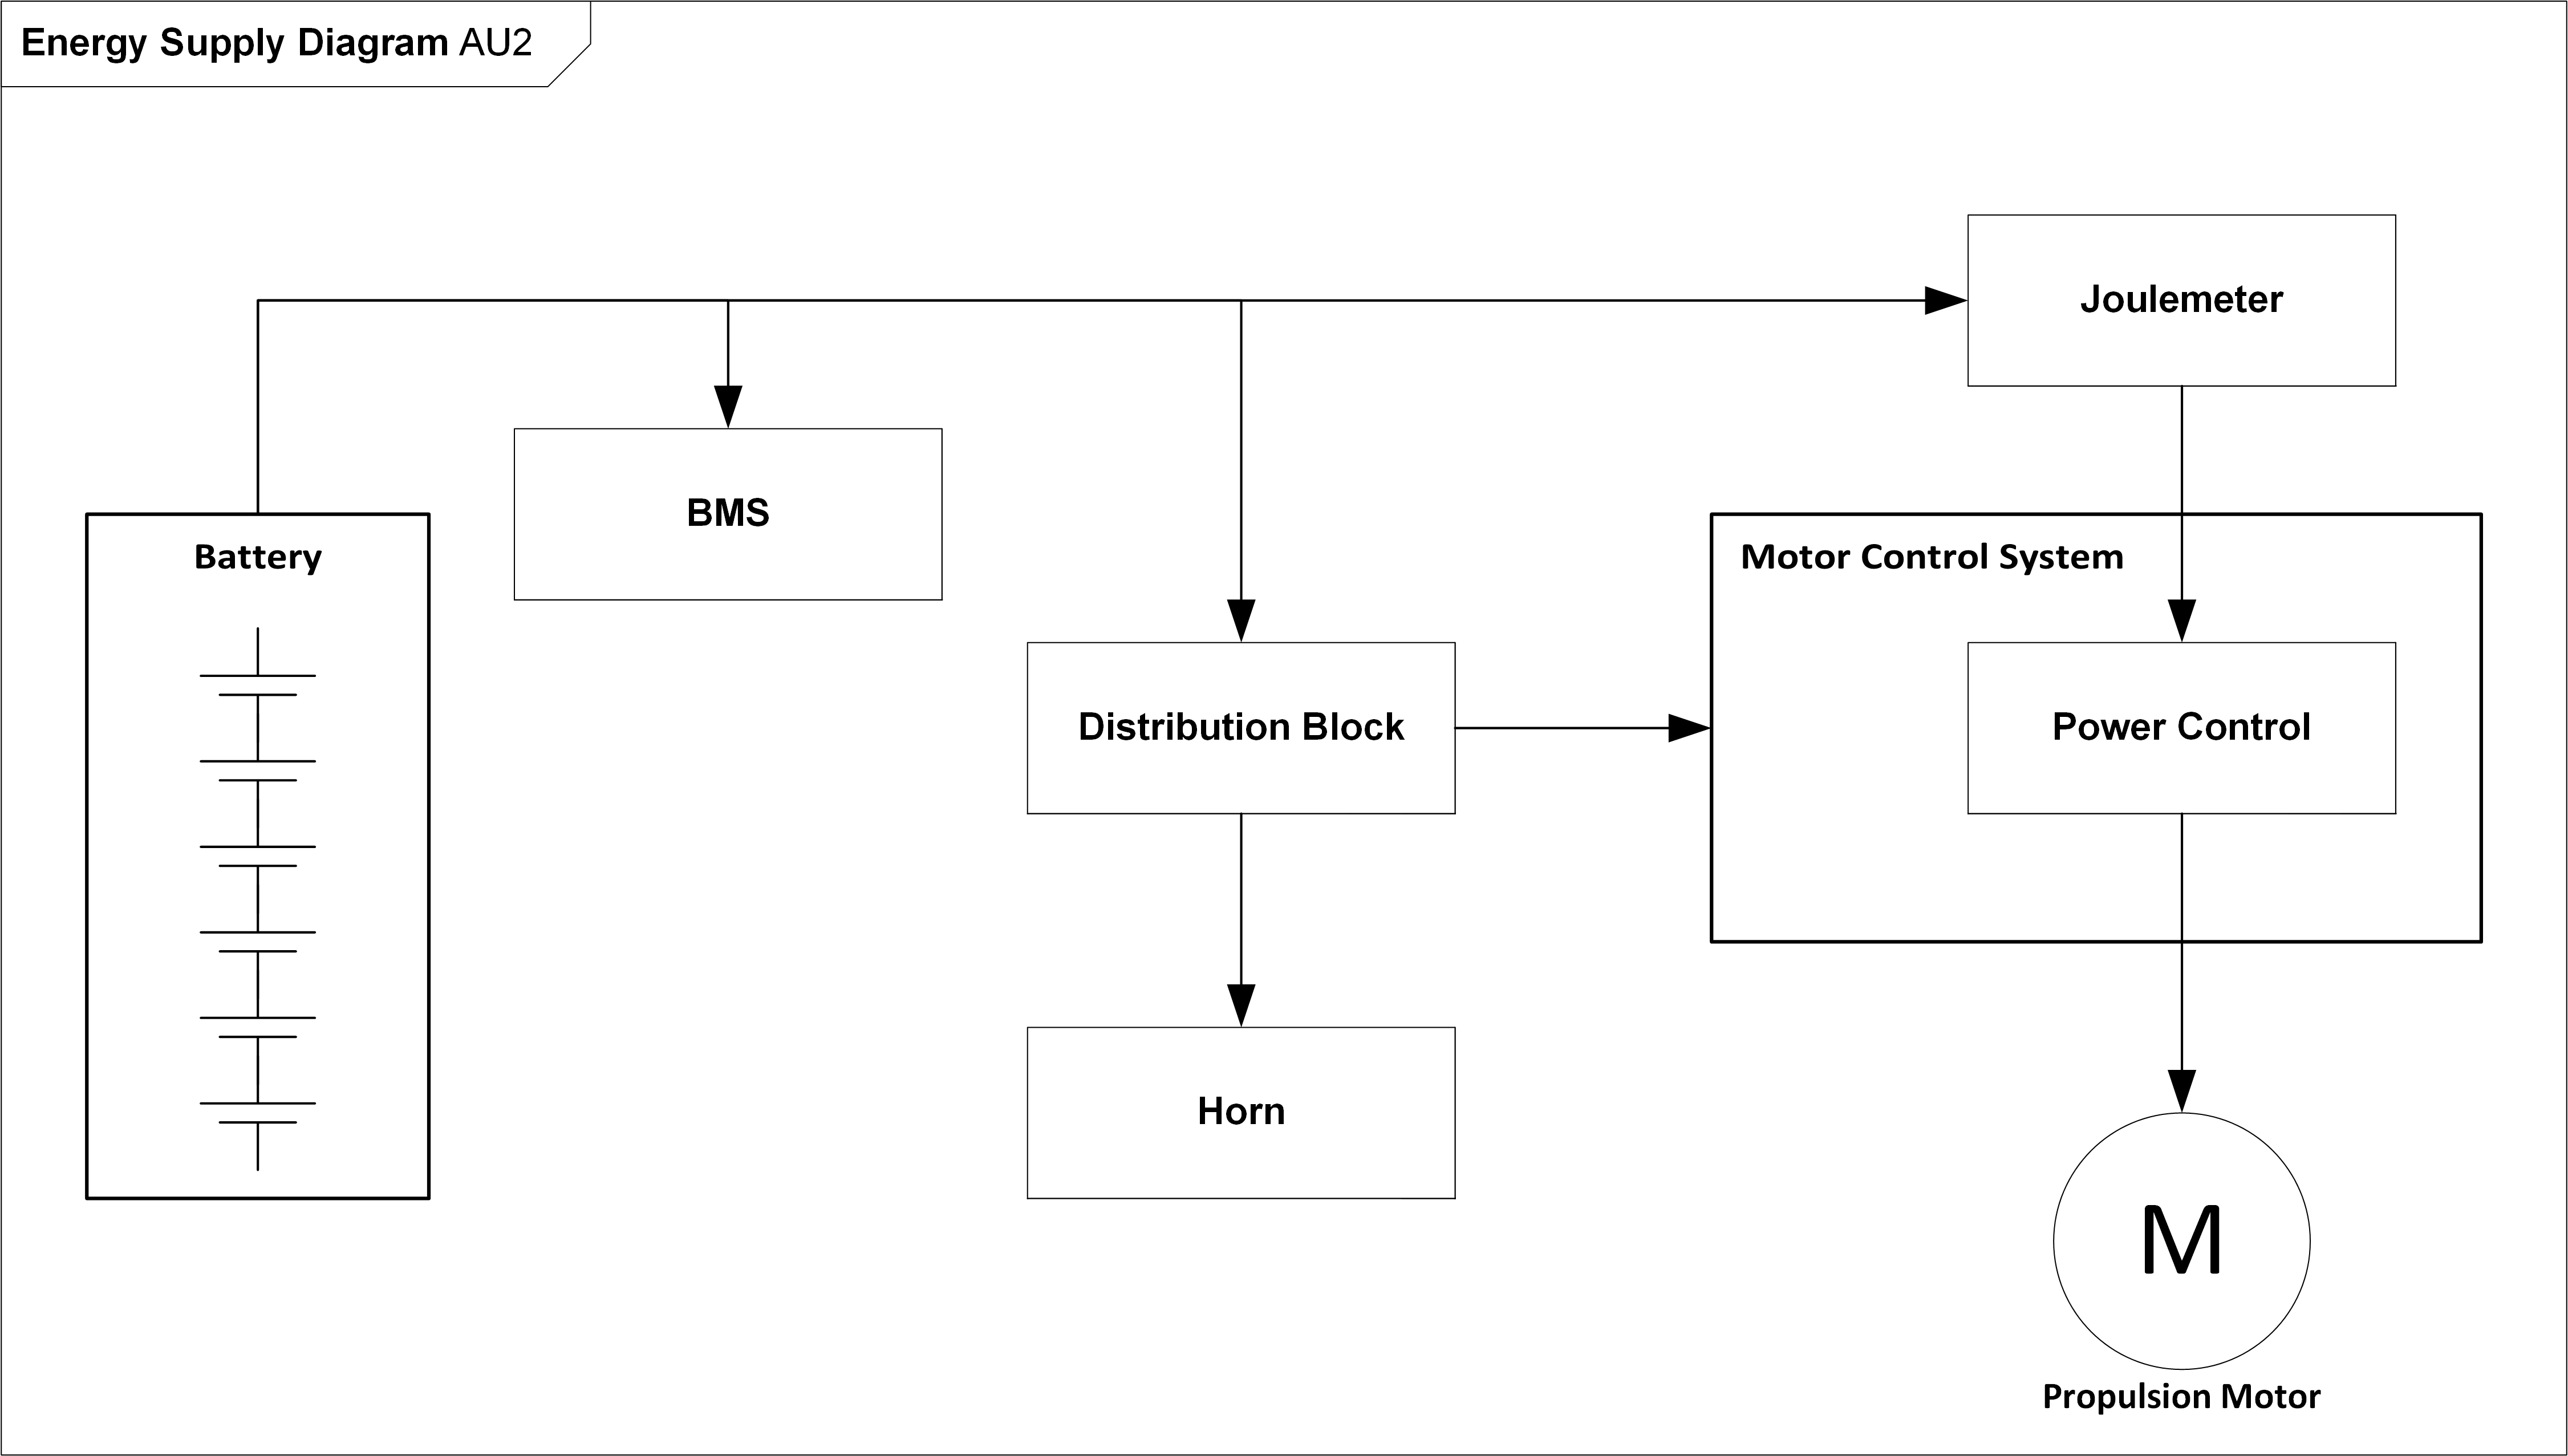
\includegraphics[width=0.9\linewidth]{Hardware/Pictures/Energy_Supply_Diagram}
	\caption{Energy Supply Diagram}
	\label{fig:Energy_supply}
\end{figure}

\subsection{Implementation}
The Shell Joulemeter is handed out during the Shell Eco-Marathon and therefore cannot be implemented beforehand. However, according to the SEM requirements the Joulemeter must be located such that the display is visible on the outside of the car. The Joulemeter itself can be implemented by using four spade connectors which can be screwed in place.

When the car is not used to compete in Shell Eco-Marathon the Joulemeter can be disconnected and the Battery can be directly connected to the Power Control Block. It should also be noted that the Joulemeter can be replaced with Rolling Road's Power-sensor - if the user wishes to test the car using the battery.